\documentclass[a4paper,11pt]{article}

% Language setting
\usepackage[english]{babel}

% Font and encoding - Good practice for PDF output
\usepackage[T1]{fontenc}
\usepackage{lmodern}

% Page size and margins
\usepackage[top=2cm,bottom=2cm,left=2.2cm,right=2.2cm,marginparwidth=1.75cm]{geometry}

% Useful packages
\usepackage{amsmath}
\usepackage{graphicx}
\usepackage{float} % Keep float for [H] or [htbp]
\usepackage[hidelinks]{hyperref} % Hidelinks removes the colored boxes
\hypersetup{colorlinks=true,allcolors=blue}

% Packages for better tables
\usepackage{booktabs} % For professional tables (\toprule, \midrule, \bottomrule)
\usepackage{array} % For table column formatting

% Graphics path (images folder is at repo root, one level up from 'rapport')
\graphicspath{{../images/}}

% Title
\title{Simple Consensus System for Distributed Locks\\
\large ICT3 Project n°2 — Shanghai Jiao Tong University}
\author{Alexandra Baron \and Maria Stivala \and Mathis Liens \and Arnaud Brisset \and Charles Pelong\and Baptiste Halçaren}
\date{October 2025}

\begin{document}

\maketitle

% University logo - Placed AFTER title and smaller
\begin{figure}[htbp]
\centering

\includegraphics[width=0.4\linewidth]{shanghai-jiao-tong-university.png}
\end{figure}

\begin{abstract}
This report presents the design and implementation of a simple consensus system for managing distributed locks using a leader-follower architecture. The implementation, realized in \texttt{Java} using sockets, guarantees strong consistency: all mutation operations (\emph{lock}/\emph{unlock}) are validated by the leader and then replicated to all followers, while read requests (\emph{own}) are served locally by any server. We describe the project's objective, the methodology used, the system architecture, and the code structure. Finally, we present experimental results and discuss the system's limitations.
\end{abstract}

\section{Context and Objective}
As part of the ICT3 (Information and Communication Technologies) course, the objective was to \textbf{design a simple consensus system} meeting the following requirements: (i) one leader and multiple followers; (ii) a replicated \textit{map} (key $\rightarrow$ owner) for the locks; (iii) multiple clients able to \texttt{tryLock}, \texttt{tryUnLock}, and \texttt{ownTheLock}; (iv) \textbf{all} mutation operations (\texttt{LOCK}/\texttt{UNLOCK}) must be routed to the leader; (v) read operations (\texttt{OWN}) can be served locally by followers; (vi) the leader updates its map and \textbf{propagates an update proposal} to all followers.

The core challenge is ensuring data consistency, guaranteeing that all servers have the same view of who owns which lock, especially during concurrent client requests.

\section{Method and Implementation Choices}
We opted for a \textbf{leader-follower architecture} built on Java TCP sockets. This approach was chosen for its explicit control over the network communication and its suitability for the project's requirements.

\begin{itemize}
    \item \textbf{Reasoning (Technology Choice)}: Java was selected as suggested in the project subject. Its built-in socket libraries (\texttt{java.net}) and robust concurrency utilities (\texttt{java.util.concurrent}) are well-suited for this task. The \texttt{ExecutorService} provides an efficient way to manage client connections without the overhead of creating a new thread for every request.

    \item \textbf{Minimalist Text Protocol}: We designed a simple, human-readable text protocol (e.g., \texttt{LOCK,<lockName>,<clientId>}). This choice simplifies debugging and implementation compared to a binary protocol, which would require more complex serialization/deserialization logic.

    \item \textbf{Request Routing}: Followers act as simple routers for write operations, forwarding \texttt{LOCK}/\texttt{UNLOCK} requests to the leader. This design decision is central to ensuring consistency, as it establishes the leader as the single point of truth (or "single-writer") for all state changes, preventing split-brain scenarios.

    \item \textbf{Synchronous Replication}: The leader uses a synchronous \texttt{SYNC}/\texttt{ACK} model for replication. When the leader approves a \texttt{LOCK} or \texttt{UNLOCK} operation, it sends a \texttt{SYNC} message to all followers. It (conceptually) waits for an \texttt{ACK} from each follower before confirming success to the client.
    
    \item \textbf{Reasoning (Consistency)}: This synchronous approach provides strong consistency. When a client receives a \texttt{SUCCESS} response, it has a guarantee that the state change has been accepted by the leader *and* replicated to its followers. The alternative, asynchronous replication, would be faster for the client but would create a window where a client could read stale data from a follower.

    \item \textbf{Simple Error Handling}: The system relies on socket timeouts (5-10s) and explicit response codes (\texttt{SUCCESS}/\texttt{FAIL}/\texttt{NONE}/\texttt{ERROR}/\texttt{TIMEOUT}). This provides basic robustness against network delays or unresponsive servers without implementing a complex failure-detection and leader-election protocol, which was deemed outside the project's scope.
\end{itemize}

\section{Data Flow and Architecture}
The system's functional architecture is centralized around the leader, which serializes all state changes. The interactions are as follows:

\begin{enumerate}
    \item \textbf{Write Operation (LOCK/UNLOCK)}: Client $\rightarrow$ Follower $\rightarrow$ Leader $\rightarrow$ All Followers (SYNC/ACK) $\rightarrow$ Leader $\rightarrow$ Follower $\rightarrow$ Client. If the client contacts the leader directly, the follower forwarding steps are skipped.
    \item \textbf{Read Operation (OWN)}: Client $\rightarrow$ (Any) Server $\rightarrow$ Client. This operation is handled locally by whichever server receives it to ensure low latency.
\end{enumerate}

This flow is illustrated in Figure \ref{fig:mermaid}, which shows the sequence of network calls for both a write (\texttt{LOCK}) and a read (\texttt{OWN}) operation.

% Note: This figure requires you to export your Mermaid diagram to "images/mermaid-flow.png"
\begin{figure}[htbp]
    \centering
    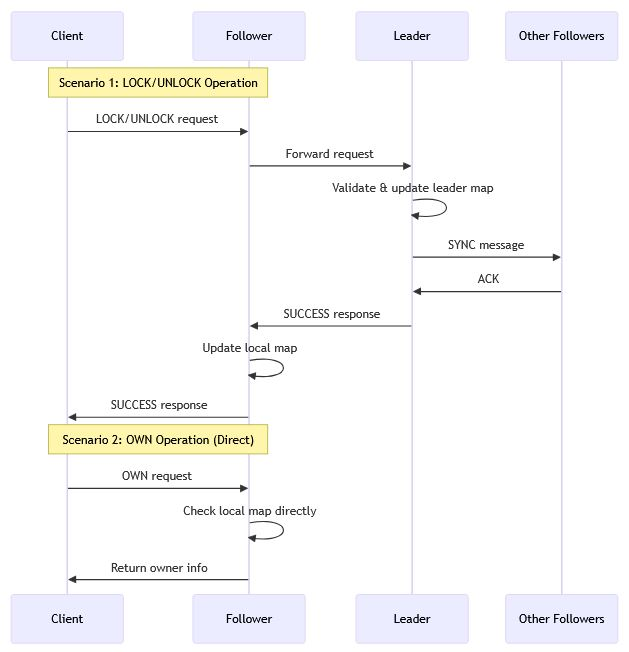
\includegraphics[width=0.85\linewidth]{images/mermaid.JPG}
    \caption{Sequence diagram of system operations (LOCK and OWN).}
    \label{fig:mermaid}
\end{figure}

\section{Structure of the Code}
The project consists of three main Java classes:

\begin{itemize}
    \item \textbf{\texttt{Client.java}}: This class provides the client-facing API: \texttt{tryLock}, \texttt{tryUnLock}, and \texttt{ownTheLock}. Each operation opens a new, short-lived socket, sends its request message via \texttt{sendMsg()}, and reads the single-line response from the server.

    \item \textbf{\texttt{DistributedLockTest.java}}: A test suite that uses a \texttt{FixedThreadPool} to simulate concurrent clients. These clients connect to different servers in the cluster (the leader at 10.0.2.3, and followers at 10.0.2.4 / 10.0.2.5) to verify concurrent lock acquisition, owner-reading, and lock release.
    
    \item \textbf{\texttt{Server.java}}: This is the core class, capable of running in either "leader" or "follower" mode. It uses a \texttt{CachedThreadPool} to handle each incoming connection in a separate thread (\texttt{handleClient()}).
        \begin{itemize}
            \item \texttt{handleClientRequest()}: Parses client messages (\texttt{LOCK}, \texttt{UNLOCK}, \texttt{OWN}) and routes them to \texttt{processRequest()}.
            \item \texttt{processRequest()}: This \texttt{synchronized} method is the main logic gate.
                \begin{itemize}
                    \item If \textbf{isLeader}, it calls \texttt{handleLeaderRequest()} to enforce business rules, update the local \texttt{lockMap}, and trigger replication via \texttt{notifyFollowers()}.
                    \item If \textbf{isFollower}, it calls \texttt{handleFollowerRequest()}.
                \end{itemize}
            \item \texttt{handleFollowerRequest()}:
                \begin{itemize}
                    \item For \texttt{OWN}, it reads its local \texttt{lockMap} and returns the value (fast, local read).
                    \item For \texttt{LOCK}/\texttt{UNLOCK}, it forwards the request to the leader via \texttt{forwardToLeader()} and returns the leader's response.
                \end{itemize}
            \item \texttt{notifyFollowers()}: The leader iterates through its list of followers, submitting a new task to the thread pool for each one to send a \texttt{SYNC} message in parallel and wait for an \texttt{ACK}.
            \item \texttt{handleSyncMessage()}: Triggered when a message starts with \texttt{SYNC,}. This is how a follower receives updates. It calls \texttt{processSync()} to apply the change to its local \texttt{lockMap} and sends back an \texttt{ACK}.
        \end{itemize}
\end{itemize}

\subsection*{Business Rules (Enforced by Leader)}
\begin{itemize}
    \item \textbf{Preemption (LOCK)}: Success if the lock (key) does not exist in the \texttt{lockMap}. Failure otherwise.
    \item \textbf{Release (UNLOCK)}: Success if the lock (key) exists *and* the caller's \texttt{clientId} matches the one stored in the map. Failure otherwise.
    \item \textbf{Read (OWN)}: Any client can query the owner. The request is handled by any server and returns the owner's \texttt{clientId} or \texttt{NONE} if the lock does not exist.
\end{itemize}

\section{Communication Protocol and Error Handling}
The system uses a simple, text-based, comma-delimited protocol.

\subsection*{Client-Server Messages}
\begin{table}[htbp]
\centering
\caption{Client-Server and Inter-Server Protocol}
\label{tab:protocol}
\begin{tabular}{@{}lll@{}}
\toprule
\textbf{Type} & \textbf{Format} & \textbf{Description} \\
\midrule
Client $\rightarrow$ Server & \texttt{LOCK,\$name,\$client} & Lock acquisition request \\
Client $\rightarrow$ Server & \texttt{UNLOCK,\$name,\$client} & Lock release request \\
Client $\rightarrow$ Server & \texttt{OWN,\$name,\$client} & Read owner request \\
Leader $\rightarrow$ Followers & \texttt{SYNC,\$cmd,\$name,\$client} & State replication (e.g., SYNC,LOCK,...) \\
Followers $\rightarrow$ Leader & \texttt{ACK} & Acknowledgment of SYNC \\
Followers $\rightarrow$ Leader & \texttt{REGISTER,\$ip:\$port} & Follower registration on startup \\
\bottomrule
\end{tabular}
\end{table}

\subsection*{Server Responses and Error Handling}
Server responses to the client are simple, single-word strings, as shown in Table \ref{tab:responses}. This provides basic robustness. Timeouts are implemented on socket operations (e.g., 10s for forwarding to leader, 5s for SYNC) to prevent threads from hanging indefinitely on network issues.

\begin{table}[htbp]
\centering
\caption{Server Response Codes}
\label{tab:responses}
\begin{tabular}{@{}ll@{}}
\toprule
\textbf{Response Code} & \textbf{Meaning} \\
\midrule
\texttt{SUCCESS} & Operation (LOCK/UNLOCK) succeeded. \\
\texttt{FAIL} & Operation (LOCK/UNLOCK) failed (e.g., lock taken, not owner). \\
\texttt{NONE} & \texttt{OWN} request returned no owner for the lock. \\
\texttt{<ClientID>} & \texttt{OWN} request returned the current lock owner. \\
\texttt{ERROR} & A generic connection or processing error occurred. \\
\texttt{TIMEOUT} & A network operation (e.g., forwarding) timed out. \\
\bottomrule
\end{tabular}
\end{table}

\section{Experimental Results}
The following figures illustrate the system in operation, using three virtual machines as specified in the \texttt{README.md}.

\begin{figure}[H]
\centering
\includegraphics[width=0.9\linewidth]{images/Capture_connection des 3 serveurs.JPG}
\caption{Initialization of the leader (10.0.2.3) and the two followers (10.0.2.4, 10.0.2.5).}
\end{figure}

\begin{figure}[H]
\centering
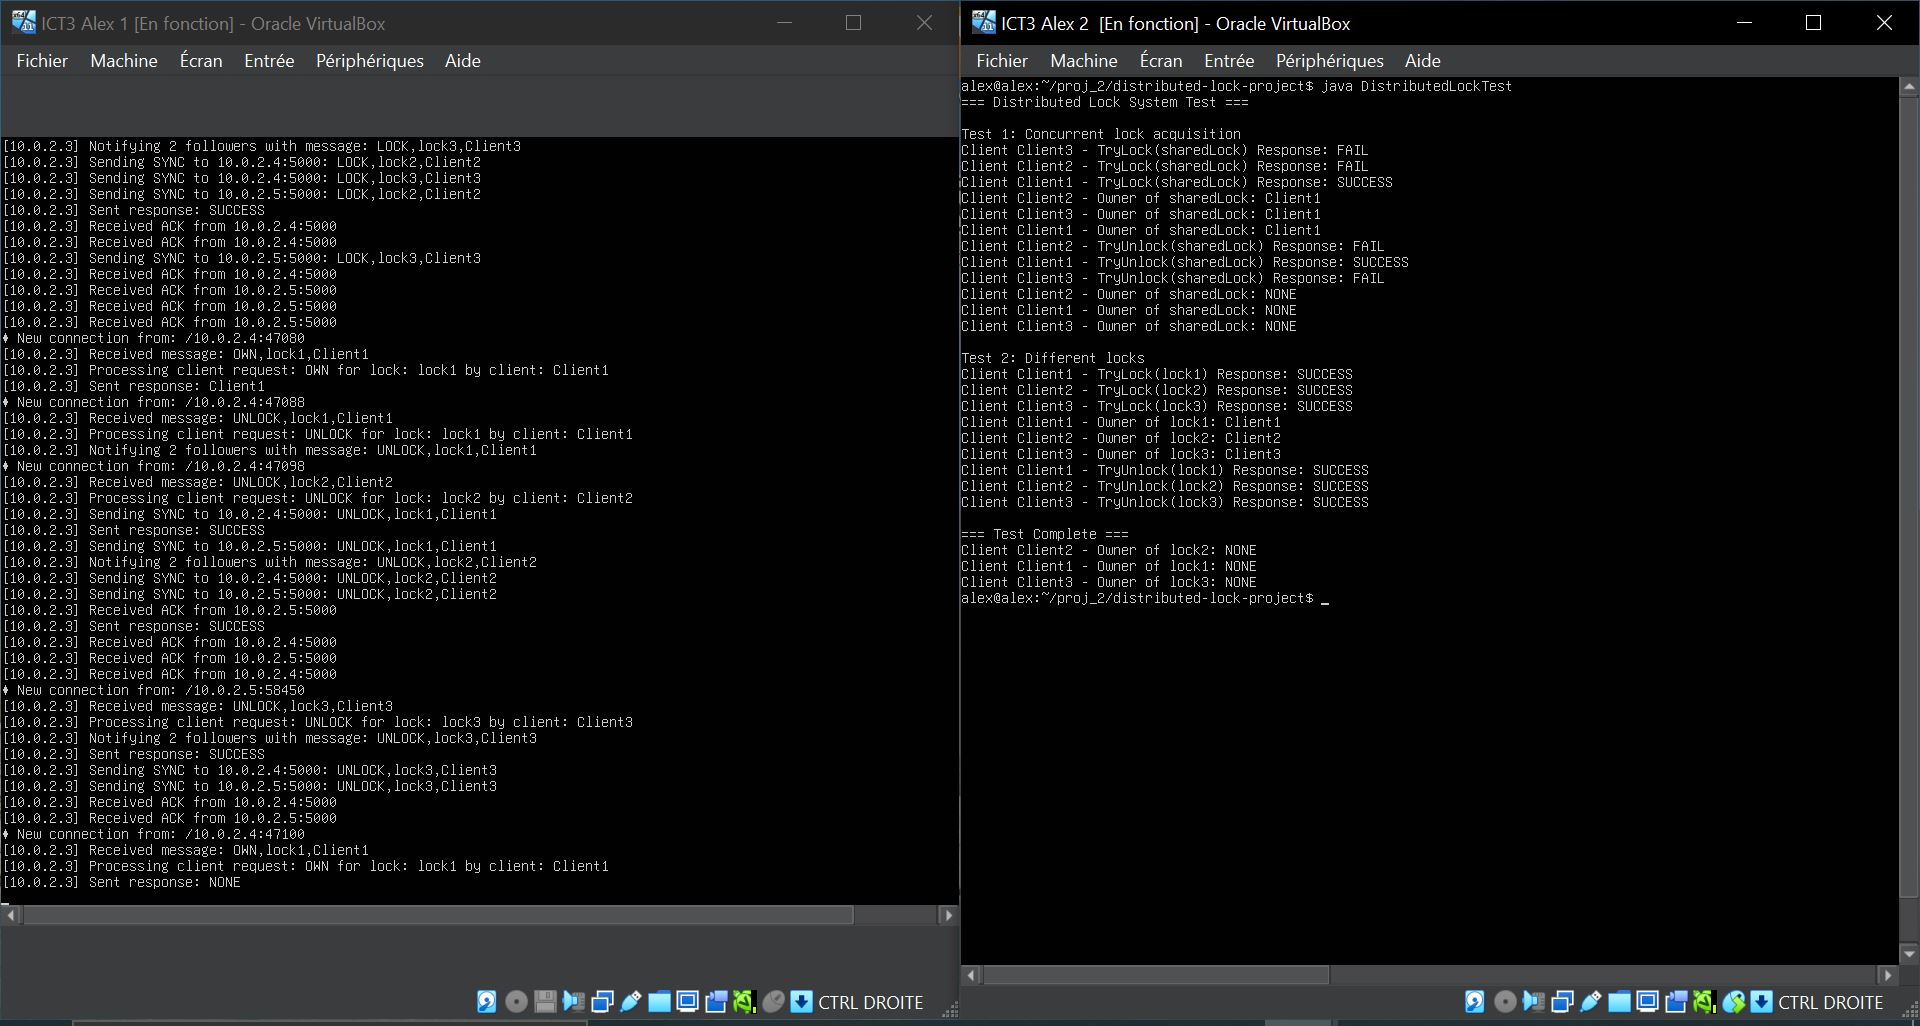
\includegraphics[width=0.9\linewidth]{images/Capture_distributed_lock_test.JPG}
\caption{Execution of \texttt{DistributedLockTest}: concurrent acquisitions, reads, and releases.}
\end{figure}

\begin{figure}[H]
\centering
\includegraphics[width=0.9\linewidth]{images/Capture_ connection de deux clients.JPG}
\caption{Concurrent connection of two clients to two different servers (a follower and the leader).}
\end{figure}

\subsection*{Observations}
\begin{itemize}
    \item The test results (Figure 2) show that for a single lock, only one client's \texttt{LOCK} request succeeds, while concurrent attempts from other clients correctly fail (returning \texttt{FAIL}).
    \item \texttt{OWN} requests, even when sent to followers, correctly return the ID of the lock owner or \texttt{NONE} after the lock is released.
    \item This confirms that the \texttt{SYNC} replication mechanism successfully maintains a consistent state map across the leader and all followers.
\end{itemize}

\section{Limitations and Future Work}
While functional, this implementation has several limitations that could be addressed in future work.
\begin{itemize}
    \item \textbf{Pending State}: The project subject mentioned checking if a request is "pending". Our implementation is fully synchronous from the follower's perspective (forward $\rightarrow$ wait for response). A more advanced implementation could have the follower track "pending" requests it has forwarded but not yet received a \texttt{SYNC} confirmation for.
    \item \textbf{Hard-coded Configuration}: The leader's address (10.0.2.3) and the list of followers are hard-coded in \texttt{Server.java}. This is inflexible. A better solution would use a configuration file or command-line arguments to define the cluster topology.
    \item \textbf{Fault Tolerance}: The system has a single point of failure (SPOF): the leader. If the leader server crashes, the system can no longer process any \texttt{LOCK} or \texttt{UNLOCK} requests. A robust system would require a fault-tolerance mechanism, such as leader election (e.g., using Paxos or Raft), which was outside the scope of this project.
    \item \textbf{Network}: Communication is unencrypted (plaintext), and there is no client authentication. This is insecure for a production environment.
\end{itemize}

\section{Conclusion}
We have successfully implemented a distributed lock system that fulfills the core requirements of the project. It uses a leader-follower architecture with a simple Java socket protocol to manage \texttt{LOCK}, \texttt{UNLOCK}, and \texttt{OWN} operations. The system ensures strong consistency by routing all write operations through the leader and using synchronous replication to update followers. Tests demonstrate the system's correctness in handling concurrent requests and maintaining a consistent state. This project serves as a solid foundation for understanding consensus and could be extended to include more advanced features like dynamic configuration and leader election.

\section{Appendix}

\end{document}
